\documentclass[11pt]{article}

\usepackage{amsmath,textcomp,amssymb,geometry,graphicx,enumerate,amsthm}
\usepackage{algpseudocode}
\usepackage[linesnumbered,ruled,vlined]{algorithm2e}
\usepackage{threeparttable, adjustbox, booktabs}

\def\endproofmark{$\Box$}
\newtheorem{theorem}{Theorem}[section]
\newtheorem{lemma}[theorem]{Lemma}
\theoremstyle{definition}
\newtheorem{definition}{Definition}[section]
\theoremstyle{remark}
\newtheorem*{remark}{Remark}
\usepackage{tikz}
\usetikzlibrary{positioning}

\renewcommand\arraystretch{1.5}

%-----------------------------------------------------------------------------------

% Title information
\title{CS 170 HW 12}
\author{Daniel Deng, SID 3034543526}
\pagestyle{myheadings}
\date{}

%-----------------------------------------------------------------------------------

\begin{document}
\maketitle

\section{Study Group}
\begin{enumerate}
\item[(a)] Auston Lin, SID 3034554056
\item[(b)] Yes
\end{enumerate}
\clearpage

\section{Reduction to 3-Coloring}
\begin{enumerate}
\item[(a)] $\forall x_i$, add edges $(x_i, base), (\neg x_i, base), (x_i, \neg x_i)$ to the graph. Connections to the ``base'' vertex ensures that $x_i$ and $\neg x_i$ can only be ```true'' or ``false''. Connection between $x_i$ and $\neg x_i$ ensures that if one is ``true'' the other must be ``false''.

\item[(b)] (Right grey vertex = color 1 $\implies$ $\exists$ left grey vertex = color 1)

\begin{proof}
After setting the right grey vertex to be color 1 and assigning its immediate neighbors, we get two cases after pruning the domains

\adjustbox{width=0.4\textwidth}{
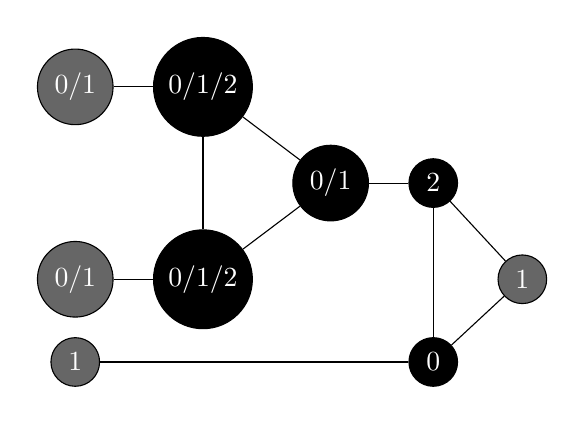
\begin{tikzpicture}[
grey/.style={circle, draw, fill=black!60, text=white},
black/.style={circle, draw, fill=black, text=white},
]

\matrix[row sep=1mm,column sep=5mm] {
\node[grey] (a1) {0/1}; & \node[black] (a2) {0/1/2}; \\
&&\node[black] (b1) {0/1}; & \node[black] (b2) {2}; \\
\node[grey] (c1) {0/1}; & \node[black] (c2) {0/1/2};&&&\node[grey] (c3) {1}; \\
\node[grey] (d1) {1}; &&& \node[black] (d2) {0};\\
};

\path 
(a1) edge (a2)
(a2) edge (c2)
(a2) edge (b1)
(b1) edge (b2)
(b1) edge (c2)
(b2) edge (c3)
(b2) edge (d2)
(c1) edge (c2)
(d1) edge (d2)
(d2) edge (c3)
;
\end{tikzpicture}
}
\adjustbox{width=0.4\textwidth}{
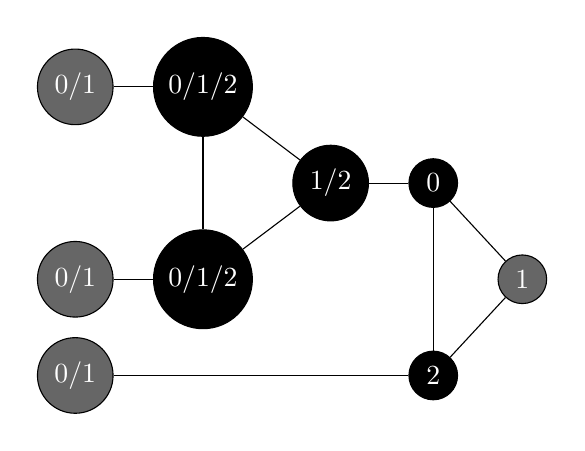
\begin{tikzpicture}[
grey/.style={circle, draw, fill=black!60, text=white},
black/.style={circle, draw, fill=black, text=white},
]

\matrix[row sep=1mm,column sep=5mm] {
\node[grey] (a1) {0/1}; & \node[black] (a2) {0/1/2}; \\
&&\node[black] (b1) {1/2}; & \node[black] (b2) {0}; \\
\node[grey] (c1) {0/1}; & \node[black] (c2) {0/1/2};&&&\node[grey] (c3) {1}; \\
\node[grey] (d1) {0/1}; &&& \node[black] (d2) {2};\\
};

\path 
(a1) edge (a2)
(a2) edge (c2)
(a2) edge (b1)
(b1) edge (b2)
(b1) edge (c2)
(b2) edge (c3)
(b2) edge (d2)
(c1) edge (c2)
(d1) edge (d2)
(d2) edge (c3)
;
\end{tikzpicture}
}

The left case already has one of the left grey vertices be of color 1. For the right case, we perform another round of assignment, and get another two cases

\adjustbox{width=0.4\textwidth}{
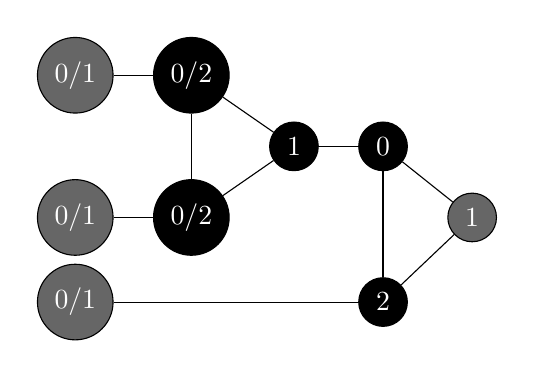
\begin{tikzpicture}[
grey/.style={circle, draw, fill=black!60, text=white},
black/.style={circle, draw, fill=black, text=white},
]

\matrix[row sep=1mm,column sep=5mm] {
\node[grey] (a1) {0/1}; & \node[black] (a2) {0/2}; \\
&&\node[black] (b1) {1}; & \node[black] (b2) {0}; \\
\node[grey] (c1) {0/1}; & \node[black] (c2) {0/2};&&&\node[grey] (c3) {1}; \\
\node[grey] (d1) {0/1}; &&& \node[black] (d2) {2};\\
};

\path 
(a1) edge (a2)
(a2) edge (c2)
(a2) edge (b1)
(b1) edge (b2)
(b1) edge (c2)
(b2) edge (c3)
(b2) edge (d2)
(c1) edge (c2)
(d1) edge (d2)
(d2) edge (c3)
;
\end{tikzpicture}
}
\adjustbox{width=0.4\textwidth}{
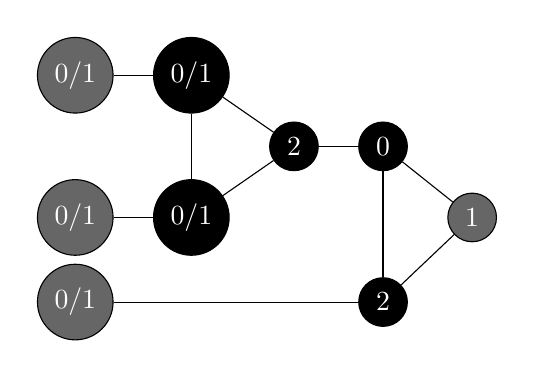
\begin{tikzpicture}[
grey/.style={circle, draw, fill=black!60, text=white},
black/.style={circle, draw, fill=black, text=white},
]

\matrix[row sep=1mm,column sep=5mm] {
\node[grey] (a1) {0/1}; & \node[black] (a2) {0/1}; \\
&&\node[black] (b1) {2}; & \node[black] (b2) {0}; \\
\node[grey] (c1) {0/1}; & \node[black] (c2) {0/1};&&&\node[grey] (c3) {1}; \\
\node[grey] (d1) {0/1}; &&& \node[black] (d2) {2};\\
};

\path 
(a1) edge (a2)
(a2) edge (c2)
(a2) edge (b1)
(b1) edge (b2)
(b1) edge (c2)
(b2) edge (c3)
(b2) edge (d2)
(c1) edge (c2)
(d1) edge (d2)
(d2) edge (c3)
;
\end{tikzpicture}
}

In both cases, since at least one of the black vertices in the left triangular structure has to take color 0, one of the two top left grey vertices must take color 1.

Therefore, the gray vertex on the right is assigned the color 1 only if one of the gray vertices on the left is assigned the color 1 given the constraint.
\end{proof}
\clearpage

\item[(c)]
\textbf{Algorithm Description:} Given a 3-SAT instance with $n$ variables and $m$ clauses. 

First, for each clause, construct a gadget such that the left grey vertices correspond to the variables or negations of variables in the clause.

Then, connect all left grey vertices from all gadgets to ``Base'', and all right grey vertices to ``Base'' and ``False''. 

Finally, pairwise connect the left grey vertices from all gadgets such that one of the left grey vertex in a pair corresponds to variable $x_i$ and the other corresponds to $\neg x_i$. 

Define ``True'' = color 1, ``False'' = color 2, and ``Base'' = color 3 and find a 3-Coloring assignment for the constructed graph. If the graph is not 3-colorable, the 3-SAT instance is not satisfiable; otherwise, the color assignment of the left grey vertices is the true/false assignment of the variables and variable negations in the clauses.

\textbf{Proof of Correctness:} First, note that in the construct graph all right grey vertices are forced to have color 1 due to their connection to both ``Base'' and ``False'' (based on \textit{observation(i)}) and any pair of left grey vertices corresponding to $x_i$ and $\neg x_i$ but be that one is assigned color 1 and the other is assigned color 0 (as shown in \textit{part(a)}).
\begin{itemize}
\item If the 3-SAT instance has a satisfying assignment, it means that at least one of the variables (or variable negations) in all clauses is true. This would mean that in the corresponding 3-Coloring graph, at least one of the left grey vertex in any gadget has color 1. Based on \textit{observation(ii)}, there is a valid coloring for all black vertices in all gadgets. Therefore, 3-Coloring will also have a satisfying assignment.

\item If the 3-Coloring graph has a satisfying assignment, since all right grey vertices have color 1, based on what we've shown in \textit{part(b)}, at least one of the left grey vertices must also have color 1 in all gadgets. This means that at least one variable (or variable negation) is true in all corresponding clauses, indicating that the 3-SAT instance can also be satisfied by the assignment.
\end{itemize}

Therefore, the reduction is correct.
\end{enumerate}
\clearpage

\section{Multiway Cut}
\begin{enumerate}
\item[(a)]
The problem of finding $F_i$ can be reduced the minimum s,t cut problem. Assuming that $G$ is undirected and unweighted, we can construct a flow graph from $G$ that replaced each undirected edge with a forward and a backward directed edge with edge capacities 1. We then add a dummy sink node that contains an in-edge with infinity edge capacity from each special vertex except $s_i$. Run the minimum s,t cut algorithm, which is polynomial time, on the flow graph, and we will find $F_i$ in polynomial time. This algorithm is correct because the minimum cut must result in all non-$s_i$ special vertices occurring in the same set as $t$ as the newly added edges with infinite edge capacity will never be included be included in the min-cut.

\item[(b)] 
Each edge in $F^*$ must only appear in 2 different $F_i^*$ (one for each endpoint) since one vertex cannot appear in multiple $C_i$. 

$|F_i| \leq |F_i^*|$ because $F_i$ is the minimum cut that separates $s_i$ from other special vertices; therefore, $|F_i^*|$ can only be as small as $|F_i|$.

\item[(c)]
\begin{align*}
F = \cup_i F_i \implies |F| \leq \sum_i |F_i| \\
\text{Each edge in $F^*$ appear in 2 $F_i^*$} \implies 2|F^*| = \sum_i |F_i^*| \\
|F_i| \leq |F_i^*| \implies |F| \leq \sum_i |F_i| \leq \sum_i |F_i^*| = 2|F^*| \\
\end{align*}
\end{enumerate}
\clearpage

\section{Project}
\begin{enumerate}
\item[(a)] A set of $n$ igloo polishing tasks such that each task has the same duration of $d$, the same profit $p$, and the same 1440 deadline has the trivial solution of picking any sequence of tasks in whatever order as long as the total time does not exceed 1440. Since the order to execute identical tasks is irrelevant as long as we maximize the number of tasks to be completed by the end of the day, we can pick the tasks in whatever way we want, and the solution is always trivial.

\item[(b)]
\begin{enumerate}
\item[(i)] The optimal sequence of igloos to polish is: $4\to1\to2$.
\item[(ii)] Yes. The optimal tasks to be completed would be $2,3,4,5$ in whatever order, since we can schedule the tasks into the 100-minute interval as tightly as possible without the constraint of individual deadlines.
\end{enumerate}

\item[(c)]
\begin{enumerate}
\item[(i)]
\begin{itemize}
\item Igloo 1: Duration = 10, Deadline = 1, Profit = 10
\item Igloo 2: Duration = 2, Deadline = 2, Profit = 2
\end{itemize}

The greedy solver would choose the sequence $1 \to 2$, since task 1 has a higher profit than task 2, resulting in an overall profit of $1$ since it is past deadline for task 1 by 9 minutes, whereas the optimal sequence is $2 \to 1$, resulting in an overall profit of $2$.

\item[(ii)]
\begin{itemize}
\item Igloo 1: Duration = 10, Deadline = 1, Profit = 1
\item Igloo 2: Duration = 2, Deadline = 2, Profit = 10
\end{itemize}

The greedy solver would choose the sequence $1\to 2$, since task 1 has an earlier deadline, resulting in a total profit of 0, whereas the optimal sequence is $2 \to 1$, resulting in a total profit of 10.
\end{enumerate}
\end{enumerate}
\end{document}


